\section{Model Error}

We generally want to minimize the estimation error $\ell(\hat{f}(x), f^*(x))$, since we do not know $f^*$ we can not actually compute this value. Instead, we usually observe $y_i = f^*(x_i) + \epsilon_i$. For each observed sample we can compute the \textbf{prediction error} $\ell(\hat{f}(x), y)$, in fact we are often interested in the average prediction error or \textbf{generalization error}:
$$R(\hat{f}) := \E_{x,y}[\ell(\hat{f}(x), y)] = \E_x[\ell(\hat{f}(x), f^*(x))] + \epsilon$$

The generalization error computed over all possible $(x,y)$ pairs weighted by how likely each is. 

The training loss is often to optimistic to approximate the generalization error. To get a better approximation we split our data into training and test set. 

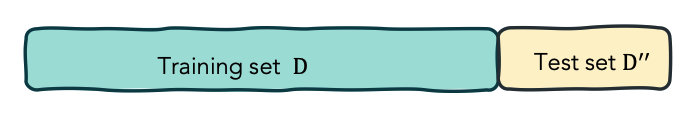
\includegraphics[width=\columnwidth]{train-test-split.png}

By only using the training set to fit our model, we have the test data to get a better estimate of the generalization error.

\subsection{Cross-Validation}

When choosing between different model, we might choose the model with the lowest test set error, this may introduce a systematic bias. To prevent this from happening we can split the training set again, creating a validation set. Now the idea is to choose the model with the best validation error and use the test set only to get the estimate for the generalization error.

Setting aside so much data can be wasteful. So we introduce \textbf{$k$-fold cross-validation}

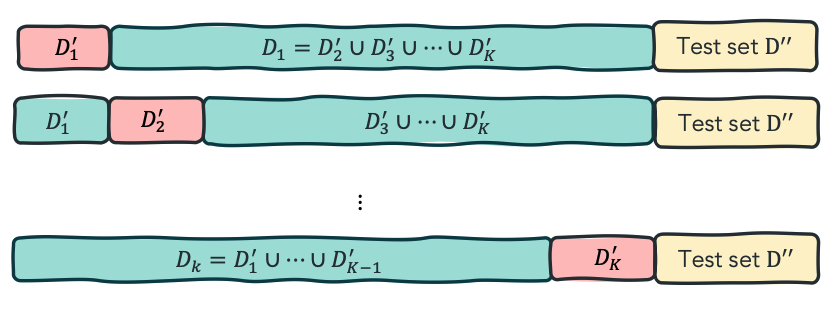
\includegraphics[width=\columnwidth]{cross-validation.png}

We proceed as follows:
\begin{enumerate}
	\item For all folds $k = 1,..., K$: 
		\begin{enumerate}
			\item Train $\hat{f}_k$ on $D' - D'_k$
			\item Compute val. error $R_k = \frac{1}{|D'_k|} \sum_{x,y} \ell(\hat{f}_k(x), y)$
		\end{enumerate}
	\item Compute cross-validation error $CV = \frac{1}{K} \sum_{i=1}^K R_i$
	\item Pick model with lowest cross-validation error $CV$
	\item Evaluate the model using the test set $D''$
\end{enumerate}

For $K$ very large, we can get the best approximation, if $K = |D'|$ we call it leave-one-out cross-validation (LOOCV).

\subsection{Model Complexity}

Model complexity is closely related to training and generalization error.

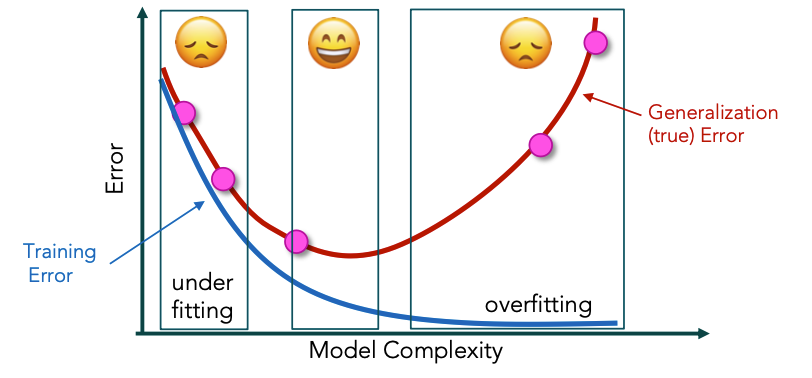
\includegraphics[width=\columnwidth]{overfitting.png}

\subsection{Bias and Variance}

For different datasets $D_1,...,D_K$ we define:
\begin{itemize}
	\item \textbf{Bias} - distance of the average model $\bar{f} = \frac{1}{K} \sum_{i=1}^K \hat{f}_i$ to the ground truth $\E_x[\ell(\bar{f}(x), f^*(x))]$
	\item \textbf{Variance} - average distance of the models to the average model $\E_x[\frac{1}{K} \sum_{i=1}^K \ell(\hat{f}_i(x), \bar{f}(x))]$
\end{itemize}

\begin{center}
	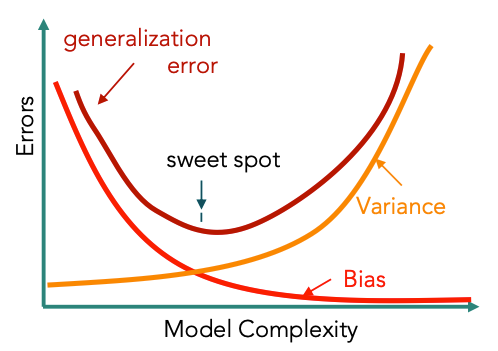
\includegraphics[width=0.8\columnwidth]{bias-variance-tradeoff.png}
\end{center}